\chapter{Programes per a la calculadora \textsf{HP Prime}}\label{sec:progs-HP}
\index{HP Prime@\textsf{HP Prime}}\index{HP Prime@\textsf{HP Prime}!funcions}

\lstset{
	language=HPPRIME,
	basicstyle=\small\sf,
	numbers=left,
	frame=lines
}

Es donen en aquest apèndix una sèrie de programes per a la calculadora \textsf{HP Prime} de Hewlett-Packard, els quals són d'interès per resoldre problemes tractats en aquest llibre.

\begin{center}
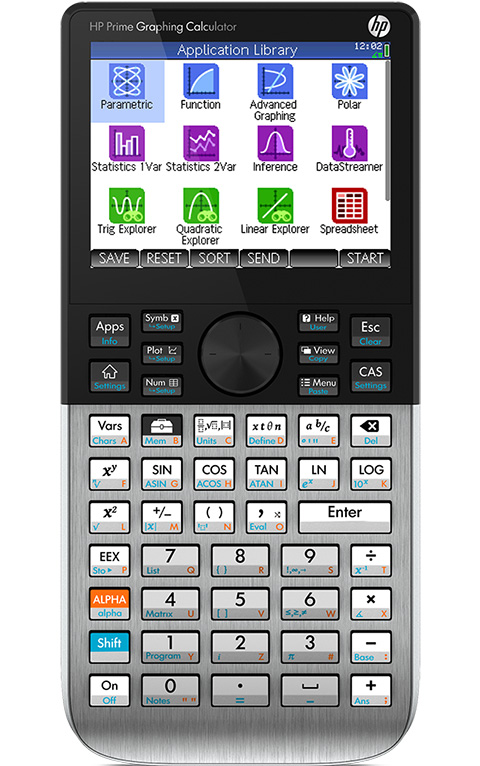
\includegraphics[scale=0.45]{Ape-HP-Prime.jpg}
\end{center}

Aquesta calculadora disposa d'un emulador per a PC que pot descarregar-se de la pàgina de Hewlett-Packard: \href{http://www.hpprime.de/en/category/6-downloads}{www.hpprime.de/en/category/6-downloads}.

\section{Electrotècnia}\label{sec:HP_ELC}

La funció \funsfbs{Z\_Sèrie} utilitza l'equació \eqref{eq:z_serie} per obtenir la impedància sèrie d'una llista d'impedàncies $\cmplx{Z}_1, \cmplx{Z}_2, ...$; les impedàncies poden ser indistintament reals o complexes.

\index{HP Prime@\textsf{HP Prime}!funcions!zserie@\funsfbs{Z\_Sèrie}}
\begin{lstlisting}[caption={HP Prime --- Funció Z\_Sèrie}]
EXPORT Z_Sèrie(z)
// z:impedàncies {Z1, Z2,...} → impedància sèrie
BEGIN
  RETURN ΣLIST(z);
END;
\end{lstlisting}

La funció \funsfbs{Z\_Paraŀlel} obté la impedància paraŀlel  d'una llista d'impedàncies $\cmplx{Z}_1, \cmplx{Z}_2, ...$; les impedàncies poden ser indistintament reals o complexes. S'utilitza una variant de l'equació \eqref{eq:z_parallel}, la qual dona una millor precisió numèrica.

\index{HP Prime@\textsf{HP Prime}!funcions!zserie@\funsfbs{Z\_Sèrie}}
\begin{lstlisting}[caption={HP Prime --- Funció Z\_Paraŀlel}]
EXPORT Z_Paraŀlel(z)
// z:impedàncies {Z1, Z2,...} → impedància paraŀlel
BEGIN
  RETURN ΠLIST(z)/ΣLIST(ΠLIST(z)/z);
END;
\end{lstlisting}

La funció \funsfbs{Millman} utilitza l'equació \eqref{eq:millman} per obtenir la tensió $\cmplx{U}\ped{nx}$ del punt neutre $n$ d'una llista d'impedàncies connectades en estrella $\cmplx{Z}\ped{an}, \cmplx{Z}\ped{bn}, \cmplx{Z}\ped{cn}, ...$, respecte d'un punt qualsevol $x$, a partir de la llista de tensions $\cmplx{U}\ped{ax}, \cmplx{U}\ped{bx}, \cmplx{U}\ped{cx}, ...$ dels extrems d'aquestes impedàncies respecte del mateix punt $x$; les impedàncies i les tensions poden ser indistintament reals o complexes. És necessària la funció \funsfbs{Z\_Paraŀlel}, definit anteriorment.

\index{HP Prime@\textsf{HP Prime}!funcions!millman@\funsfbs{Millman}}
\begin{lstlisting}[caption={HP Prime --- Funció Millman}]
EXPORT Millman(u,z)
// u:tensions {Uax,Ubx,Ucx,...}, z:impedàncies {Zan,Zbn,Zcn,...} → tensió Unx
// n és el punt neutre de les impedàncies, i x és un punt qualsevol
BEGIN
  RETURN ΣLIST(u ./ z) * Z_Paraŀlel(z);
END;
\end{lstlisting}

La funció \funsfbs{Triangle\_a\_Estrella} utilitza l'equació \eqref{eq:Y_D} per transformar una llista de tres impedàncies connectades en triangle $\cmplx{Z}\ped{ab}$, $\cmplx{Z}\ped{bc}$ i  $\cmplx{Z}\ped{ca}$, en una llista de tres impedàncies equivalents connectades en estrella $\cmplx{Z}\ped{an}$, $\cmplx{Z}\ped{bn}$ i $\cmplx{Z}\ped{cn}$; les impedàncies poden ser indistintament reals o complexes.

\index{HP Prime@\textsf{HP Prime}!funcions!triangleaestrella@\funsfbs{Triangle\_a\_Estrella}}
\begin{lstlisting}[caption={HP Prime --- Funció Triangle\_a\_Estrella}]
EXPORT Triangle_a_Estrella(zd)
// zd:impedàncies en triangle {Zab,Zbc,Zca} → impedàncies en estrella {Zan,Zbn,Zcn}
BEGIN
  LOCAL z:=ΠLIST(zd)/ΣLIST(zd);
  RETURN {z/zd(2),z/zd(3),z/zd(1)};
END;
\end{lstlisting}

La funció \funsfbs{Estrella\_a\_Triangle} utilitza l'equació \eqref{eq:Y_D} per transformar una llista de tres impedàncies connectades en estrella $\cmplx{Z}\ped{an}$, $\cmplx{Z}\ped{bn}$ i $\cmplx{Z}\ped{cn}$, en una llista de tres impedàncies equivalents connectades en triangle $\cmplx{Z}\ped{ab}$, $\cmplx{Z}\ped{bc}$ i  $\cmplx{Z}\ped{ca}$; les impedàncies poden ser indistintament reals o complexes.

\index{HP Prime@\textsf{HP Prime}!funcions!estrellaatriangle@\funsfbs{Estrella\_a\_Triangle}}
\begin{lstlisting}[caption={HP Prime --- Funció Estrella\_a\_Triangle}]
EXPORT Estrella_a_Triangle(zy)
// zy:impedàncies en estrella {Zan,Zbn,Zcn} → impedàncies en triangle {Zab,Zbc,Zca}
BEGIN
  LOCAL z:=zy(1)*(zy(2)+zy(3))+zy(2)*zy(3);
  RETURN {z/zy(3),z/zy(1),z/zy(2)};
END;
\end{lstlisting}

La funció \funsfbs{EZS\_U} utilitza les equacions de la secció \vref{sec:EZS} per obtenir la tensió $\cmplx{U}$ d'una càrrega que absorbeix una potència $\cmplx{S}$, quan està connectada a una font de tensió $\cmplx{E}$ a través d'una impedància $\cmplx{Z}$; cadascun d'aquests valors pot ser indistintament real o complex.

\index{HP Prime@\textsf{HP Prime}!funcions!ezsu@\funsfbs{EZS\_U}}
\begin{lstlisting}[caption={HP Prime --- Funció EZS\_U},label=lst:EZSU]
EXPORT EZS_U(E,Z,S)
// E:font de tensió, Z:impedància, S:potència de la càrrega → tensió U de la càrrega
BEGIN
  LOCAL ZcS:=CONJ(Z)*S;
  LOCAL ImUe:=IM(ZcS)/ABS(E);
  LOCAL ReUe:=POLYROOT({1,-ABS(E),RE(ZcS)+ImUe^2});
  IF TYPE(ReUe(1))==3 THEN
    RETURN "No hi ha solució"; // Arrels complexes
  ELSE
    RETURN (MAX(ReUe),ImUe)*SIGN(E);
  END;
END;
\end{lstlisting}

La funció \funsfbs{kcmil\_a\_mm2} utilitza l'equació \eqref{eq:kcmil_mm2} per convertir la secció d'un conductor expressada en \unit{kcmil}, en la seva secció equivalent expressada en \unit{mm^2}.

\index{HP Prime@\textsf{HP Prime}!funcions!kcmilamm@\funsfbs{kcmil\_a\_mm2}}
\begin{lstlisting}[caption={HP Prime --- Funció kcmil\_a\_mm2}]
EXPORT kcmil_a_mm2(kcmil)
// kcmil:secció en kcmil → secció en mm²
BEGIN
  RETURN kcmil*0.506707479098;
END;
\end{lstlisting}

La funció \funsfbs{mm2\_a\_kcmil} utilitza l'equació \eqref{eq:kcmil_mm2} per convertir la secció d'un conductor expressada en \unit{mm^2}, en la seva secció equivalent expressada en \unit{kcmil}.

\index{HP Prime@\textsf{HP Prime}!funcions!mmakcmil@\funsfbs{mm2\_a\_kcmil}}
\begin{lstlisting}[caption={HP Prime --- Funció mm2\_a\_kcmil}]
EXPORT mm2_a_kcmil(mm2)
// mm2:secció en mm² → secció en kcmil
BEGIN
  RETURN mm2/0.506707479098;
END;
\end{lstlisting}

La funció \funsfbs{AWG\_a\_mm2} utilitza l'equació \eqref{eq:awg_mm2} per convertir la secció d'un conductor expressada segons el seu número AWG, en la seva secció equivalent expressada en \unit{mm^2}.

\index{HP Prime@\textsf{HP Prime}!funcions!awgamm@\funsfbs{AWG\_a\_mm2}}
\begin{lstlisting}[caption={HP Prime --- Funció AWG\_a\_mm2}]
EXPORT AWG_a_mm2(AWG)
// AWG:número AWG → secció en mm²
// Cal entrar 0, -1, -2 i -3 en el cas dels números AWG 1/0, 2/0, 3/0 i 4/0
BEGIN
  RETURN 53.4751207321/(92^(AWG/19.5));
END;
\end{lstlisting}

La funció \funsfbs{mm2\_a\_AWG} utilitza l'equació \eqref{eq:mm2_awg} per convertir la secció d'un conductor expressada en \unit{mm^2}, en la seva secció equivalent expressada segons el seu número AWG; la conversió és aproximada, ja que els números AWG prenen valors discrets.

\index{HP Prime@\textsf{HP Prime}!funcions!mmaawg@\funsfbs{mm2\_a\_AWG}}
\begin{lstlisting}[caption={HP Prime --- Funció mm2\_a\_AWG}]
EXPORT mm2_a_AWG(mm2)
// mm2:secció en mm² → número AWG més proper
// Els resultats 0, -1, -2 i -3 són equivalents als números AWG 1/0, 2/0, 3/0 i 4/0
BEGIN
  RETURN ROUND(4.31245284200*LN(53.4751207321/mm2),0);
END;
\end{lstlisting}


La funció \funsfbs{Triangle\_a\_Fasors} obté els tres fasors $\cmplx{U}\ped{AB}$, $\cmplx{U}\ped{BC}$ i $\cmplx{U}\ped{CA}$ que formen un triangle de tensions fase-fase, a partir de les longituds dels tres costats d'aquest triangle $|\cmplx{U}\ped{AB}|$, $|\cmplx{U}\ped{BC}|$ i $|\cmplx{U}\ped{CA}|$. Es pren $\cmplx{U}\ped{AB}$ com a fasor de referència.

\index{HP Prime@\textsf{HP Prime}!funcions!triangleafasors@\funsfbs{Triangle\_a\_Fasors}}
\begin{lstlisting}[caption={HP Prime --- Funció Triangle\_a\_Fasors},label=lst:TriFas]
EXPORT Triangle_a_Fasors(u)
// u:triangle de tensions {Uab,Ubc,Uca} → fasors de tensió {Uab,Ubc,Uca}
// La tensió Uab es pren com el fasor de referència (angle igual a zero)
BEGIN
  LOCAL 𝜑:=Triangle_Solver.SSS(u(1),u(3),u(2));
  RETURN {u(1),u(2)*(-1,0)*(1,∡𝜑(2)),u(3)*(-1,0)/(1,∡𝜑(3))};
END;
\end{lstlisting}

La funció \funsfbs{FN\_a\_FF} obté els fasors de les tres tensions fase-fase $\cmplx{U}\ped{AB}$, $\cmplx{U}\ped{BC}$ i $\cmplx{U}\ped{CA}$, corresponents als fasors de les tres tensions fase-neutre
$\cmplx{U}\ped{AN}$, $\cmplx{U}\ped{BN}$ i $\cmplx{U}\ped{CN}$.

\index{HP Prime@\textsf{HP Prime}!funcions!fnaff@\funsfbs{FN\_a\_FF}}
\begin{lstlisting}[caption={HP Prime --- Funció FN\_a\_FF}, label=lst:FNaFF]
EXPORT FN_a_FF(u)
// u:tensions fase-neutre {Uan,Ubn,Ucn} → tensions fase-fase {Uab,Ubc,Uca}
BEGIN
  RETURN {u(1)-u(2),u(2)-u(3),u(3)-u(1)};
END;
\end{lstlisting}

La funció \funsfbs{FF\_a\_FN} obté els fasors de les tres tensions fase-neutre $\cmplx{U}\ped{AN}$, $\cmplx{U}\ped{BN}$ i $\cmplx{U}\ped{CN}$, corresponents a tres impedàncies $\cmplx{Z}\ped{AN}$, $\cmplx{Z}\ped{BN}$ i $\cmplx{Z}\ped{CN}$ connectades en estrella a  les tres tensions fase-fase
$\cmplx{U}\ped{AB}$, $\cmplx{U}\ped{BC}$ i $\cmplx{U}\ped{CA}$.

\index{HP Prime@\textsf{HP Prime}!funcions!ffafn@\funsfbs{FF\_a\_FN}}
\begin{lstlisting}[caption={HP Prime --- Funció FF\_a\_FN}, label=lst:FFaFN]
EXPORT FF_a_FN(u,z)
// u:tensions fase-fase {Uab,Ubc,Uca}, z:impedàncies {Zan,Zbn,Zcn} → tensions
// fase-neutre {Uan,Ubn,Ucn}
BEGIN
  RETURN {u(1)/z(2)-u(3)/z(3),u(2)/z(3)-u(1)/z(1),u(3)/z(1)-u(2)/z(2)}*Z_Paraŀlel(z);
END;
\end{lstlisting}

La funció \funsfbs{FF\_a\_FG} obté els fasors de les tres tensions fase-neutre $\cmplx{U}\ped{AG}$, $\cmplx{U}\ped{BG}$ i $\cmplx{U}\ped{CG}$ que tenen el punt neutre G en el baricentre del triangle format pels fasors de  les tres tensions fase-fase
$\cmplx{U}\ped{AB}$, $\cmplx{U}\ped{BC}$ i $\cmplx{U}\ped{CA}$. És un cas particular de la funció anterior, quan les tres impedàncies són idèntiques.

\index{HP Prime@\textsf{HP Prime}!funcions!ffafg@\funsfbs{FF\_a\_FG}}
\begin{lstlisting}[caption={HP Prime --- Funció FF\_a\_FG}, label=lst:FFaFG]
EXPORT FF_a_FG(u)
// u:tensions fase-fase {Uab,Ubc,Uca} → tensions fase-G {Uag,Ubg,Ucg}
// G és el baricentre del triangle de tensions fase-fase
BEGIN
  RETURN {u(1)-u(3),u(2)-u(1),u(3)-u(2)}/3;
END;
\end{lstlisting}

La funció \funsfbs{ABC\_a\_A012} utilitza l'equació \eqref{eq:c_sim_mat1} per obtenir els tres fasors de seqüència
$\cmplx{A}_0$, $\cmplx{A}_1$ i  $\cmplx{A}_2$ corresponents als tres fasors $\cmplx{A}$, $\cmplx{B}$ i $\cmplx{C}$.

\index{HP Prime@\textsf{HP Prime}!funcions!abcaa012@\funsfbs{ABC\_a\_A012}}
\begin{lstlisting}[caption={HP Prime --- Funció ABC\_a\_A012}, label=lst:ABCaA012]
EXPORT ABC_a_A012(x)
// x:fasors {A,B,C} → fasors de seqüència {A0,A1,A2}
BEGIN
  LOCAL A:=[[1,1,1],[1,(-1/2,√3/2),(-1/2,-√3/2)],[1,(-1/2,-√3/2),(-1/2,√3/2)]];
  RETURN mat2list(A*list2mat(x,1)/3);
END;
\end{lstlisting}

La funció \funsfbs{A012\_a\_ABC} fa el càlcul  invers de la funció anterior, i utilitza l'equació \eqref{eq:c_sim_mat} per obtenir els tres fasors
$\cmplx{A}$, $\cmplx{B}$ i $\cmplx{C}$  corresponents als tres fasors de seqüència
$\cmplx{A}_0$, $\cmplx{A}_1$ i  $\cmplx{A}_2$.

\index{HP Prime@\textsf{HP Prime}!funcions!a012aabc@\funsfbs{A012\_a\_ABC}}
\begin{lstlisting}[caption={HP Prime --- Funció A012\_a\_ABC}, label=lst:A012aABC]
EXPORT A012_a_ABC(x)
// x:fasors de seqüència {A0,A1,A2} → fasors {A,B,C}
BEGIN
  LOCAL A:=[[1,1,1],[1,(-1/2,-√3/2),(-1/2,√3/2)],[1,(-1/2,√3/2),(-1/2,-√3/2)]];
  RETURN mat2list(A*list2mat(x,1));
END;
\end{lstlisting}

La funció \funsfbs{AN12\_a\_AB12} utilitza les equacions  \eqref{eq:c_sim_a3} i \eqref{eq:c_sim_b3} per obtenir els dos fasors de tensions de seqüència fase-fase $\cmplx{U}\ped{AB,1}$ i  $\cmplx{U}\ped{AB,2}$ a partir dels dos fasors de tensions de seqüència fase-neutre $\cmplx{U}\ped{AN,1}$ i $\cmplx{U}\ped{AN,2}$.

\index{HP Prime@\textsf{HP Prime}!funcions!an12aab12@\funsfbs{AN12\_a\_AB12}}
\begin{lstlisting}[caption={HP Prime --- Funció AN12\_a\_AB12}, label=lst:AN12aAB12]
EXPORT AN12_a_AB12(x)
// x:fasors de seqüència fase-neutre {AN1,AN2} → fasors de seqüència fase-fase {AB1,AB2}
BEGIN
  RETURN √3*{x(1)*exp(𝜋*i/6),x(2)*exp(-𝜋*i/6)};
END;
\end{lstlisting}

La funció \funsfbs{AB12\_a\_AN12} fa el càlcul invers de la funció anterior, i utilitza les mateixes equacions  \eqref{eq:c_sim_a3} i \eqref{eq:c_sim_b3} per obtenir els dos fasors de tensions de seqüència fase-neutre $\cmplx{U}\ped{AN,1}$ i $\cmplx{U}\ped{AN,2}$ a partir dels dos fasors de tensions de seqüència fase-fase $\cmplx{U}\ped{AB,1}$ i  $\cmplx{U}\ped{AB,2}$:

\index{HP Prime@\textsf{HP Prime}!funcions!ab12aan12@\funsfbs{AB12\_a\_AN12}}
\begin{lstlisting}[caption={HP Prime --- Funció AB12\_a\_AN12}, label=lst:AB12aAN12]
EXPORT AB12_a_AN12(x)
// x:fasors de seqüència fase-fase {AB1,AB2} → fasors de seqüència fase-neutre {AN1,AN2}
BEGIN
  RETURN {x(1)/exp(𝜋*i/6),x(2)/exp(-𝜋*i/6)}/√3;
END;
\end{lstlisting}


\section{Matemàtiques}

La funció \funsfbs{Interpolació\_Polinòmica} obté l'ordenada interpolada $y$ corresponent a una abscissa $x$, a partir d'un conjunt  de punts $(x_1,y_1)$, $(x_2,y_2)$, ..., $(x\ped{n},y\ped{n})$. S'utilitza una interpolació polinòmica, obtenint el mateixos resultats que amb el mètode descrit en la secció \vref{sec:poli_lagr}; el grau del polinomi és igual a $n-1$.

\index{HP Prime@\textsf{HP Prime}!funcions!interpolaciopolinomica@\funsfbs{Interpolació\_Polinòmica}}
\begin{lstlisting}[caption={HP Prime --- Funció Interpolació\_Polinòmica}]
EXPORT Interpolació_Polinòmica(dades,x)
// dades:[[x1,y1], x:abscissa → ordenada y interpolada
//        [x2,y2]
//        .......
//        [xn,yn]]
BEGIN
  RETURN POLYEVAL(polynomial_regression(dades,rowDim(dades)-1),x);
END;
\end{lstlisting}


La funció \funsfbs{Interpolació\_Polinòmica\_2dim} obté el valor interpolat $z$ corresponent a un punt $(x, y)$, a partir d'un conjunt de punts $(x\ped{1}, x\ped{2}, ... x\ped{n})$, d'un conjunt de punts $(y\ped{1}, y\ped{2}, ... y\ped{m})$, i d'una matriu de valors $(z\ped{11}, z\ped{12}, ..., z\ped{1n})$,
$(z\ped{21}, z\ped{22}, ..., z\ped{2n})$, ..., $(z\ped{m1}, z\ped{m2}, ..., z\ped{mn})$. S'utilitzen  interpolacions polinòmiques, obtenint els mateixos resultats que amb el mètode descrit en la secció \vref{sec:poli_lagr}; el grau dels polinomis és igual a $n-1$ i $m-1$.
És necessària la funció \funsfbs{Interpolació\_Polinòmica}, definit anteriorment.

\index{HP Prime@\textsf{HP Prime}!funcions!interpolaciopolinomica2dim@\funsfbs{Interpolació\_Polinòmica\_2dim}}
\begin{lstlisting}[caption={HP Prime --- Funció Interpolació\_Polinòmica\_2dim}]
EXPORT Interpolació_Polinòmica_2dim(dades,x,y)
// dades:[[0,   x1,  x2, ...  xn], x, y → z interpolada
//        [y1, z11, z12, ... z1n]
//        [y2, z21, z22, ... z2n]
//        .......................
//        [ym, zm1, zm2, ... zmn]]
BEGIN
  LOCAL c:=colDim(dades);
  LOCAL r:=rowDim(dades);
  LOCAL d:=[[0,0],[0,0]];
  LOCAL z:=[[0,0],[0,0]];
  LOCAL k;
  d(-1):=dades({{1,2},{1,c}});
  FOR k FROM 2 TO r DO
    d(-2):=dades({{k,2},{k,c}});
    z(k-1,2):=Interpolació_Polinòmica(d,x);
  END;
  z(-1):=TRN(dades({{2,1},{r,1}}));
  RETURN Interpolació_Polinòmica(z,y);
END;
\end{lstlisting}

La funció \funsfbs{Regla\_dels\_Trapezis} utilitza l'equació  \eqref{eq:trap-uneven} per obtenir la integral entre $x_1$ i $x_n$ d'un conjunt  de punts $(x_1,y_1)$, $(x_2,y_2)$, ..., $(x\ped{n},y\ped{n})$, utilitzant la regla dels trapezis.

\index{HP Prime@\textsf{HP Prime}!funcions!regladelstrapezis@\funsfbs{Regla\_dels\_Trapezis}}
\begin{lstlisting}[caption={HP Prime --- Funció Regla\_dels\_Trapezis}]
EXPORT Regla_dels_Trapezis(dades)
// dades:[[x1,y1] → Integral de x1 a xn
//        [x2,y2]
//        .......
//        [xn,yn]]
BEGIN
  LOCAL k;
  LOCAL a:=0;
  LOCAL n:=rowDim(dades)-1;
  FOR k FROM 1 TO n DO
    a:=a+(dades(k+1,2)+dades(k,2))*(dades(k+1,1)-dades(k,1));
  END;
  RETURN a/2;
END;
\end{lstlisting}




